
\section{Introduction}

Event recognition and detection in videos has hugely benefited from the
introduction of recent large-scale datasets \cite{THUMOS,UCF101,Karpathy_CVPR14,MED11} and models.
However, this is mainly confined to the domain of single-person actions
where the videos contain one actor performing a primary activity.
Another equally important problem is event recognition in
videos with multiple people. In our work, we present a new model
and dataset for this specific setting.

\begin{figure}[ht!]
\begin{center}
  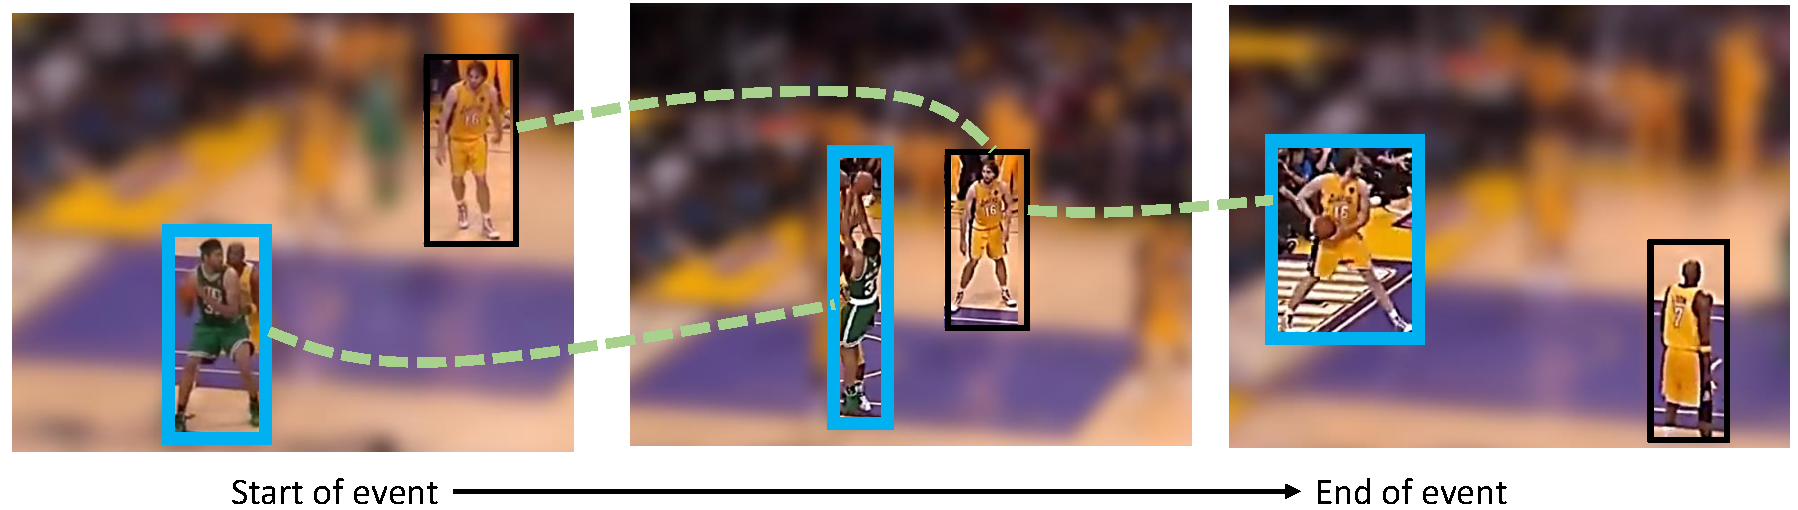
\includegraphics[width=3.5 in]{images/pull_figure_v2_cropped.pdf}
\end{center}
\caption{To recognize multi-person events, it is necessary to observe the right
person at the right instant. Here, we can identify the
event to be a ``2-pointer" by observing the shooter at the time of the shot.
Similarly, we can declare the shot to be ``successful" by looking at the
person throwing the ball into play at the end. Our model uses a similar approach to detect
an event by switching focus to the most releavant person at each instant of the video.}
\label{fig:pull_figure}
\end{figure}

Videos captured in sports arenas, market places or other outdoor areas
often contain multiple people interacting with each other.
However, the events in these videos are often
dominated by a smaller subset. For instance, a ``shot" in a sport
or ``shop-lifting" in a market is determined by one or two key people.
In such settings, apart from recognizing the event it is also important
to isolate the key actors. This is a significant challenge which
differentiates multi-person videos from single-person videos.

Observing the right people at the right time could hold the cue to
understanding an entire event. Furhter, identifying the people responsible for
the event is an interesting task in its own right.  It is also desirable to
learn a model which does not require annotations for these people during
training. The model should automatically ``attend" to the key actors while recognizing an event.

Recently, Recurrent Neural Network (RNN) models have been quite successful in
using ``attention" \cite{Bahdnau_arxiv14,Xu_arxiv15,Yao_arxiv15} for aligning
elements from an input sequence to those of an output sequence. In these settings,
the input sequence remains fixed at all times and the model chooses from this
fixed input at each instant. However, the use of such attention based RNNs
poses two challenges in our setting:
1. The set of person detections varies from one frame to the other and
2. The model needs to adapt attention according to the phase of the event as
shown in Fig.~\ref{fig:pull_figure}. This presents interesting choices
for the attention model.

While person detections vary from frame to frame, the people in the event remain
consistent throughout the video. They can be tracked across all frames and each
person-track can be treated as a separate sequence. This leads to better RNN
based representations for each person.  The attention model is then tasked with
selecting the most releavant track at each time-step in the event.  We also
analyze another variant of the method without tracking and present results for
both methods. Apart from event recognition, we also provide a quantitative
analysis of the attention results generated by our models.

To evaluate our model, we require a large dataset of multi-person activities.
Multi-person datasets like \cite{Ryoo_ICCV09,VIRAT,Choi_ICCV09} are usually restricted to fewer videos.
Further, to evaluate event detection, it is desirable to have temporal annotations in long
untrimmed videos. An easily accessible source of good quality data is
available in multi-player sports like basketball.
Hence, we propose a new dataset of basketball events with time-stamp annotations for
all occurrences of $11$ different events across $257$ videos each $1.5$ hours
long in length.  This dataset is comparable to the THUMOS \cite{THUMOS}
detection dataset in terms of number of annotations and contains longer videos
catering to a multi-person setting.

In summary, the contributions of our are paper are as follows.  First, we
introduce a new  large-scale basketball event dataset with 14K dense temporal
annotations for long video sequences.  Second, we show that our method
outperforms state-of-the-art methods for the standard tasks of classifying
isolated clips and of temporally localizing events within longer, untrimmed
videos.  Third, we show that our method learns to attend to the relevant
players, despite never being told which players are relevant in the training
set.
